\documentclass[fleqn]{ieej-report2}% documentclassの宣言で処理エンジンを指定する。
\usepackage{amsmath,amssymb,bm}% ams-LaTeXの色々を使う
\usepackage{txfonts}
\usepackage[dvipdfmx]{graphicx,color}% 
\usepackage{nidanfloat}% 2段ぶち抜きの図を下に入れる,2段ぶち抜きの図と1段以内の図が同頁に共存するために必要
%その他のusepackageは以下に書く。
%
% 参照いろいろ(ieej-tec2の内容から外れると思うので直接書き。要望あればieej-tec2.clsに移します)
\def\tabref#1{\tablename\ref{#1}}
\def\figref#1{\figurename\ref{#1}}
\def\secref#1{\ref{#1}節}
\def\formref#1{\eqref{#1}式}
%
%%%%%%%%%%%%%%%% preambleここまで %%%%%%%%%%%%%%%%
%
\begin{document}
%
%%%%%%%%%%%%%%%% ここから本文 %%%%%%%%%%%%%%%%
%
\section{大見出}

\subsection{中見出}

\subsubsection{小見出}
本文□(MS明朝 $+$ Times)□□□□□□□□□□□□□
□□□□5□□□□\scalebox{0.5}[1]{1}\scalebox{0.5}[1]{0}□□□□\scalebox{0.5}[1]{1}\scalebox{0.5}[1]{5}□□□□\scalebox{0.5}[1]{2}\scalebox{0.5}[1]{0}□□□□\scalebox{0.5}[1]{2}\scalebox{0.5}[1]{5}□
□□□□□□□□□。
□□□□□□□,□□□□□□□□□□□□□□□□□□□□□□。
□□□□□□□□□□□□□,□□□□□□□□□□□□□□□□□□。

\section{大見出}

\subsection{中見出}

\subsubsection{小見出}


中見出_段落□□□□□□□□
□□□□□□□□□□□□□□□□□□□□□□□□□□□□□□
引用文献\cite{IEEJformat}□□引用文献\cite{bib2,bib3}□□引用文献\cite{bib4,bib5,bib6,bib7}□□□□□□□□□。

本文□□□□□□□□□□□□□□□□□□□□□□□
□□□□5□□□□\scalebox{0.5}[1]{1}\scalebox{0.5}[1]{0}□□□□\scalebox{0.5}[1]{1}\scalebox{0.5}[1]{5}□□□□\scalebox{0.5}[1]{2}\scalebox{0.5}[1]{0}□□□□\scalebox{0.5}[1]{2}\scalebox{0.5}[1]{5}□
□□□□□□□□□□□□□□□□□□□□□□□□□□□□□□□□□□□□□□□□□□□。
\begin{enumerate}
\item
□□□□□□□□□□□□□□□□□□□□□□□□□□□□□□□□□□□□。
\item
□□□□□□□□□□□□□□□□□□□□□□□□□□□□□□□□□□□□。
\end{enumerate}

中見出_段落□□□□□□□□□□□□□□□□□□□□□□□□□□□□□□□□□□□□□□
□□□□□□□□□□□□□□□□□□□□□□□□□□□□□□□□□□□□。

\subsubsection{小見出}
小見出_段落□□□□□□□□□□□□□□□□□□□□□□□□□□□□□□□□□□□□□□
□□□□□□□□□□□□□□□□□□□□□□□□□□□□□□□□□□□□。

本文□□□□□□□□□□□□□□□□□□□□□□□
□□□□5□□□□\scalebox{0.5}[1]{1}\scalebox{0.5}[1]{0}□□□□\scalebox{0.5}[1]{1}\scalebox{0.5}[1]{5}□□□□\scalebox{0.5}[1]{2}\scalebox{0.5}[1]{0}□□□□\scalebox{0.5}[1]{2}\scalebox{0.5}[1]{5}□
□□□□□□□□□□□□□□□□□□□□□□□□□□□□□□□□□□□□□□□□□□□。
%
\begin{equation}
Z = X + Y \eqndotsfill{58mm}
\end{equation}
%
□□本文(字下無)□□□□□□□□□□□□□□□□□□□□□□□□□。
%
\begin{align}
Z &= X + Y \notag\\
& \qquad Z = X + Y \text{\scriptsize {数式行(続)}} \eqndotsfill{32mm}\\
\intertext{式説明□□□□□□\scalebox{0.5}[1]{1}\scalebox{0.5}[1]{0}□□□□\scalebox{0.5}[1]{1}\scalebox{0.5}[1]{5}□□□□\scalebox{0.5}[1]{2}\scalebox{0.5}[1]{0}□□□□\scalebox{0.5}[1]{2}\scalebox{0.5}[1]{5}□
□□□□□□□□□□□□□□□□□□□□□。
(ここはちゃんと実装していないので準拠でない)%
}
Z &= X + Y \times \frac AB \eqndotsfill{52mm}
\end{align}

本文□□□□□□□□□□□□□□□□□□□□□□□
□□□□5□□□□\scalebox{0.5}[1]{1}\scalebox{0.5}[1]{0}□□□□\scalebox{0.5}[1]{1}\scalebox{0.5}[1]{5}□□□□\scalebox{0.5}[1]{2}\scalebox{0.5}[1]{0}□□□□\scalebox{0.5}[1]{2}\scalebox{0.5}[1]{5}□
□□□□□□□(\tabref{tab:example}参照)。

\begin{table}[b]
\centering
\caption{タイトル}
\ecaption{Title.}
\label{tab:example}
\tabcolsep=1.5truemm
\begin{tabular}{|c|c|c|c|c|}\hline
表内文字 & \hspace{4zw} &  \hspace{4zw} &  \hspace{4zw} &  \hspace{4zw} \\\hline
Text & & & & \\\hline
& & & & \\\hline
\end{tabular}
\par
\begin{minipage}{68truemm}
\scriptsize%
図表説明(左)□□\scalebox{0.5}[1]{1}\scalebox{0.5}[1]{0}□□□□\scalebox{0.5}[1]{1}\scalebox{0.5}[1]{5}□□□□\scalebox{0.5}[1]{2}\scalebox{0.5}[1]{0}□□□□\scalebox{0.5}[1]{2}\scalebox{0.5}[1]{5}□□□□□表の左右は,75mm以内□□□□□□□□□□□。
\end{minipage}
\end{table}

本文□□□□□□□□□□□□□□□□□□□□□□□
□□□□5□□□□\scalebox{0.5}[1]{1}\scalebox{0.5}[1]{0}□□□□\scalebox{0.5}[1]{1}\scalebox{0.5}[1]{5}□□□□\scalebox{0.5}[1]{2}\scalebox{0.5}[1]{0}□□□□\scalebox{0.5}[1]{2}\scalebox{0.5}[1]{5}□□□□□□□□□□□□□□□□□□□□□□□□□□□□□□□□□□□□□□□□□□□□
□□□□□□□□□□□□□□□□□□□□□□□□□□□□□□□□□□□□□□□□□□□
□□□□□□□□□□□□□□□□□□□□□□□□□□□□□□□□□□□□□□□□□□□
□□□□□□□□□□□□□□□□□□□□□□□□□□□□□□。

本文□□□□□□□□□□□□□□□□□□□□□□□
□□□□5□□□□\scalebox{0.5}[1]{1}\scalebox{0.5}[1]{0}□□□□\scalebox{0.5}[1]{1}\scalebox{0.5}[1]{5}□□□□\scalebox{0.5}[1]{2}\scalebox{0.5}[1]{0}□□□□\scalebox{0.5}[1]{2}\scalebox{0.5}[1]{5}□
□□□□□□□(\tabref{tab:nidanfloat:example}参照)。

\begin{table*}[t]
\centering
\caption{タイトル}
\ecaption{Title.}
\label{tab:nidanfloat:example}
\tabcolsep=1.5truemm
\begin{tabular}{|c|c|c|c|c|c|c|c|c|c|c|}\hline
表内文字 & \hspace{4zw} &  \hspace{4zw} &  \hspace{4zw} &  \hspace{4zw} &  \hspace{4zw} &  \hspace{4zw} &  \hspace{4zw} &  \hspace{4zw} &  \hspace{4zw} &  \hspace{4zw} \\\hline
Text & & & & & & & & & & \\\hline
& & & & & & & & & & \\\hline
\end{tabular}
\par
% 図表説明の入れ方がハードコーディングなのはご愛嬌
\begin{minipage}{\hsize}
\scriptsize\centering%
図表説明(中央)□□□□□□表の左右は,165mm以内□□□□□□
\end{minipage}
\end{table*}

本文□□□□□□□□□□□□□□□□□□□□□□□
□□□□5□□□□\scalebox{0.5}[1]{1}\scalebox{0.5}[1]{0}□□□□\scalebox{0.5}[1]{1}\scalebox{0.5}[1]{5}□□□□\scalebox{0.5}[1]{2}\scalebox{0.5}[1]{0}□□□□\scalebox{0.5}[1]{2}\scalebox{0.5}[1]{5}□□□□□□□□□□□□□□□□□□□□□□□□□□□□□□□□□□□□□□□□□□□□
□□□□□□□□□□□□□□□□□□□□□□□□□□□□□□□□□□□□□□□□□□□□
□□□□□□□□□□□□□□□□□□□□□□□□□□□□□□□□□□□□□□□□□□□
□□□□□□□□□□□□□□□□□□□□□□□□□□□□□□。

本文□□□□□□□□□□□□□□□□□□□□□□□
□□□□5□□□□\scalebox{0.5}[1]{1}\scalebox{0.5}[1]{0}□□□□\scalebox{0.5}[1]{1}\scalebox{0.5}[1]{5}□□□□\scalebox{0.5}[1]{2}\scalebox{0.5}[1]{0}□□□□\scalebox{0.5}[1]{2}\scalebox{0.5}[1]{5}□□□□□□□□□□□□□□□□□□□□□□□□□□□□□□□□□□□□□□□□□□□□
□□□□□□□(\figref{fig:example}参照)。

%% 貼るためのeps画像をtexから作成 %%
\bgroup
\catcode37=11
\gdef\percentcharacter{%}
\egroup
\newwrite\fout%
\immediate\openout\fout=ieejtec2figure.eps%
\immediate\write\fout{\percentcharacter !PS-Adobe-3.0 EPSF-3.0}%
\immediate\write\fout{\percentcharacter\percentcharacter BoundingBox: 0 0 100 60}%
\immediate\write\fout{gsave}%
\immediate\write\fout{1 setlinewidth}%
\immediate\write\fout{gsave 0.75 setgray 0.25 setlinewidth}%
\immediate\write\fout{newpath 0 15 moveto 100 0 rlineto stroke}%
\immediate\write\fout{newpath 0 30 moveto 100 0 rlineto stroke}%
\immediate\write\fout{newpath 0 45 moveto 100 0 rlineto stroke}%
\immediate\write\fout{grestore}%
\immediate\write\fout{newpath 0 0 moveto 100 50 lineto stroke}%
\immediate\write\fout{newpath 100 0 moveto 0 0 lineto 0 60 lineto stroke}%
\immediate\write\fout{grestore}%
\immediate\write\fout{\percentcharacter\percentcharacter EOF}%
\immediate\closeout\fout%
%% ここまで %%

\begin{figure}[b]
\centering
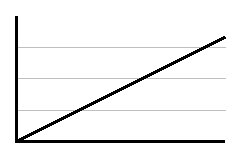
\includegraphics[width=70truemm]{ieejtec2figure.eps}
\par
(a) Graph 1.
\caption{タイトル}
\ecaption{Title.}
\label{fig:example}
\end{figure}


本文□□□□□□□□□□□□□□□□□□□□□□□
□□□□5□□□□\scalebox{0.5}[1]{1}\scalebox{0.5}[1]{0}□□□□\scalebox{0.5}[1]{1}\scalebox{0.5}[1]{5}□□□□\scalebox{0.5}[1]{2}\scalebox{0.5}[1]{0}□□□□\scalebox{0.5}[1]{2}\scalebox{0.5}[1]{5}□□□□□□□□□□□□□□□□□□□□□□□□□□□□□□□□□□□□□□□□□□□□
□□□□□□□□□□□□□□□□□□□□□□□□□□□□□□□□□□□□□□□□□□□□
□□□□□□□□□□□□□□□□□□□□□□□□□□□□□□□□□□□□□□□□□□□□
□□□□□□□□□□□□□□□□□□□□□□□□□□□□□□□□□□□□□□□□□□□
□□□□□□□□□□□□□□□□□□□□□□□□□□□□□□□□□□□□□□□□□□□
□□□□□□□□□□□□□□□□□□□□□□□□□□□□□□。

本文□□□□□□□□□□□□□□□□□□□□□□□
□□□□5□□□□\scalebox{0.5}[1]{1}\scalebox{0.5}[1]{0}□□□□\scalebox{0.5}[1]{1}\scalebox{0.5}[1]{5}□□□□\scalebox{0.5}[1]{2}\scalebox{0.5}[1]{0}□□□□\scalebox{0.5}[1]{2}\scalebox{0.5}[1]{5}□□□□□□□□□□□□□□□□□□□□□□□□□□□□□□□□□□□□□□□□□□□□
□□□□□□□□□□□□□□□□□□□□□□□□□□□□□□□□□□□□□□□□□□□□
□□□□□□□□□□□□□□□□□□□□□□□□□□□□□□□□□□□□□□□□□□□□
□□□□□□□□□□□□□□□□□□□□□□□□□□□□□□□□□□□□□□□□□□□
□□□□□□□□□□□□□□□□□□□□□□□□□□□□□□□□□□□□□□□□□□□
□□□□□□□□□□□□□□□□□□□□□□□□□□□□□□。

本文□□□□□□□□□□□□□□□□□□□□□□□
□□□□5□□□□\scalebox{0.5}[1]{1}\scalebox{0.5}[1]{0}□□□□\scalebox{0.5}[1]{1}\scalebox{0.5}[1]{5}□□□□\scalebox{0.5}[1]{2}\scalebox{0.5}[1]{0}□□□□\scalebox{0.5}[1]{2}\scalebox{0.5}[1]{5}□□□□□□□□□□□□□□□□□□□□□□□□□□□□□□□□□□□□□□□□□□□□
□□□□□□□□□□□□□□□□□□□□□□□□□□□□□□□□□□□□□□□□□□□□
□□□□□□□□□□□□□□□□□□□□□□□□□□□□□□□□□□□□□□□□□□□□
□□□□□□□□□□□□□□□□□□□□□□□□□□□□□□□□□□□□□□□□□□□
□□□□□□□□□□□□□□□□□□□□□□□□□□□□□□□□□□□□□□□□□□□
□□□□□□□□□□□□□□□□□□□□□□□□□□□□□□。

本文□□□□□□□□□□□□□□□□□□□□□□□
□□□□5□□□□\scalebox{0.5}[1]{1}\scalebox{0.5}[1]{0}□□□□\scalebox{0.5}[1]{1}\scalebox{0.5}[1]{5}□□□□\scalebox{0.5}[1]{2}\scalebox{0.5}[1]{0}□□□□\scalebox{0.5}[1]{2}\scalebox{0.5}[1]{5}□□□□□□□□□□□□□□□□□□□□□□□□□□□□□□□□□□□□□□□□□□□□
□□□□□□□□□□□□□□□□□□□□□□□□□□□□□□□□□□□□□□□□□□□□
□□□□□□□□□□□□□□□□□□□□□□□□□□□□□□□□□□□□□□□□□□□□
□□□□□□□□□□□□□□□□□□□□□□□□□□□□□□□□□□□□□□□□□□□
□□□□□□□□□□□□□□□□□□□□□□□□□□□□□□□□□□□□□□□□□□□
□□□□□□□□□□□□□□□□□□□□□□□□□□□□□□。

本文□□□□□□□□□□□□□□□□□□□□□□□
□□□□5□□□□\scalebox{0.5}[1]{1}\scalebox{0.5}[1]{0}□□□□\scalebox{0.5}[1]{1}\scalebox{0.5}[1]{5}□□□□\scalebox{0.5}[1]{2}\scalebox{0.5}[1]{0}□□□□\scalebox{0.5}[1]{2}\scalebox{0.5}[1]{5}□□□□□□□□□□□□□□□□□□□□□□□□□□□□□□□□□□□□□□□□□□□□
□□□□□□□□□□□□□□□□□□□□□□□□□□□□□□□□□□□□□□□□□□□□
□□□□□□□□□□□□□□□□□□□□□□□□□□□□□□□□□□□□□□□□□□□□
□□□□□□□□□□□□□□□□□□□□□□□□□□□□□□□□□□□□□□□□□□□
□□□□□□□□□□□□□□□□□□□□□□□□□□□□□□□□□□□□□□□□□□□
□□□□□□□□□□□□□□□□□□□□□□□□□□□□□□。

本文□□□□□□□□□□□□□□□□□□□□□□□
□□□□5□□□□\scalebox{0.5}[1]{1}\scalebox{0.5}[1]{0}□□□□\scalebox{0.5}[1]{1}\scalebox{0.5}[1]{5}□□□□\scalebox{0.5}[1]{2}\scalebox{0.5}[1]{0}□□□□\scalebox{0.5}[1]{2}\scalebox{0.5}[1]{5}□□□□□□□□□□□□□□□□□□□□□□□□□□□□□□□□□□□□□□□□□□□□
□□□□□□□□□□□□□□□□□□□□□□□□□□□□□□□□□□□□□□□□□□□□
□□□□□□□□□□□□□□□□□□□□□□□□□□□□□□□□□□□□□□□□□□□□
□□□□□□□□□□□□□□□□□□□□□□□□□□□□□□□□□□□□□□□□□□□
□□□□□□□□□□□□□□□□□□□□□□□□□□□□□□□□□□□□□□□□□□□
□□□□□□□□□□□□□□□□□□□□□□□□□□□□□□。

本文□□□□□□□□□□□□□□□□□□□□□□□
□□□□5□□□□\scalebox{0.5}[1]{1}\scalebox{0.5}[1]{0}□□□□\scalebox{0.5}[1]{1}\scalebox{0.5}[1]{5}□□□□\scalebox{0.5}[1]{2}\scalebox{0.5}[1]{0}□□□□\scalebox{0.5}[1]{2}\scalebox{0.5}[1]{5}□□□□□□□□□□□□□□□□□□□□□□□□□□□□□□□□□□□□□□□□□□□□
□□□□□□□□□□□□□□□□□□□□□□□□□□□□□□□□□□□□□□□□□□□□
□□□□□□□□□□□□□□□□□□□□□□□□□□□□□□□□□□□□□□□□□□□□
□□□□□□□□□□□□□□□□□□□□□□□□□□□□□□□□□□□□□□□□□□□
□□□□□□□□□□□□□□□□□□□□□□□□□□□□□□□□□□□□□□□□□□□
□□□□□□□□□□□□□□□□□□□□□□□□□□□□□□。

本文□□□□□□□□□□□□□□□□□□□□□□□
□□□□5□□□□\scalebox{0.5}[1]{1}\scalebox{0.5}[1]{0}□□□□\scalebox{0.5}[1]{1}\scalebox{0.5}[1]{5}□□□□\scalebox{0.5}[1]{2}\scalebox{0.5}[1]{0}□□□□\scalebox{0.5}[1]{2}\scalebox{0.5}[1]{5}□□□□□□□□□□□□□□□□□□□□□□□□□□□□□□□□□□□□□□□□□□□□
□□□□□□□□□□□□□□□□□□□□□□□□□□□□□□□□□□□□□□□□□□□□
□□□□□□□□□□□□□□□□□□□□□□□□□□□□□□□□□□□□□□□□□□□□
□□□□□□□□□□□□□□□□□□□□□□□□□□□□□□。

本文□□□□□□□□□□□□□□□□□□□□□□□
□□□□5□□□□\scalebox{0.5}[1]{1}\scalebox{0.5}[1]{0}□□□□\scalebox{0.5}[1]{1}\scalebox{0.5}[1]{5}□□□□\scalebox{0.5}[1]{2}\scalebox{0.5}[1]{0}□□□□\scalebox{0.5}[1]{2}\scalebox{0.5}[1]{5}□□□□□□□□□□□□□□□□□□□□□□□□□□□□□□□□□□□□□□□□□□□□
□□□□□□□□□□□□□□□□□□□□□□□□□□□□□□□□□□□□□□□□□□□□
□□□□□□□□□□□□□□□□□□□□□□□□□□□□□□□□□□□□□□□□□□□
□□□□□□□□□□□□□□□□□□□□□□□□□□□□□□□□□□□□□□□□□□□
□□□□□□□□□□□□□□□□□□□□□□□□□□□□□□□□□□□□□□□□□□□
□□□□□□□□□□□□□□□□□□□□□□□□□□□□□□。

本文□□□□□□□□□□□□□□□□□□□□□□□
□□□□5□□□□\scalebox{0.5}[1]{1}\scalebox{0.5}[1]{0}□□□□\scalebox{0.5}[1]{1}\scalebox{0.5}[1]{5}□□□□\scalebox{0.5}[1]{2}\scalebox{0.5}[1]{0}□□□□\scalebox{0.5}[1]{2}\scalebox{0.5}[1]{5}□□□□□□□□□□□□□□□□□□□□□□□□□□□□□□□□□□□□□□□□□□□□
□□□□□□□□□□□□□□□□□□□□□□□□□□□□□□□□□□□□□□□□□□□
□□□□□□□□□□□□□□□□□□□□□□□□□□□□□□。

\begin{thebibliography}{99}
\bibitem{IEEJformat}
原稿の書き方$\mid$一般社団法人 電気学会, \\
\verb|http://www.iee.jp/?page_id=4843| (2018年7月20日閲覧)
\bibitem{bib2}
Name : “Title English”, 雑誌名, Vol.巻数, No.号数 p.000 (発行年)\\
著書名:「タイトル」,雑誌名,Vol.巻数,No.号数 p.ページ数 (発行年)
\bibitem{bib3}
Name and Name : “Title Eng”, 雑誌名, Vol.巻数, No.号数 pp.000-000 (発行年)\\
著書名・著書名:「タイトル」,雑誌名,Vol.巻数,No.号数 pp.ページ数 (発行年)
著書名:「タイトル」,雑誌名,Vol.巻数,No.号数 pp.ページ数 (発行年)
\bibitem{bib4}
著書名:「タイトル」,雑誌名,Vol.巻数,No.号数 pp.ページ数 (発行年)
\bibitem{bib5}
著書名:「タイトル」,雑誌名,Vol.巻数,No.号数 pp.ページ数 (発行年)
\bibitem{bib6}
著書名:「タイトル」,雑誌名,Vol.巻数,No.号数 pp.ページ数 (発行年)
\bibitem{bib7}
著書名:「タイトル」,雑誌名,Vol.巻数,No.号数 pp.ページ数 (発行年)
\bibitem{bib8}
著書名:「タイトル」,雑誌名,Vol.巻数,No.号数 pp.ページ数 (発行年)
\bibitem{bib9}
著書名:「タイトル」,雑誌名,Vol.巻数,No.号数 pp.ページ数 (発行年)
\bibitem{bib10}
著書名:「タイトル」,雑誌名,Vol.巻数,No.号数 pp.ページ数 (発行年)
\bibitem{bib11}
著書名:「タイトル」,雑誌名,Vol.巻数,No.号数 pp.ページ数 (発行年)
\end{thebibliography}


\end{document}